\documentclass[8pt,a4paper]{article}
\pagestyle{plain}
\usepackage{fullpage}
\usepackage{indentfirst} %首段縮排
\usepackage[top=1.5cm, bottom=1.5cm, left=1.5cm, right=1.5cm]{geometry} %伍錫志
\usepackage{amsmath,amsthm,amsfonts,amssymb,amscd,longtable}
\usepackage{lastpage}
\usepackage{enumerate}
\usepackage{fancyhdr}
\usepackage{mathrsfs}
\usepackage{mathtools}
\usepackage{longtable}
\usepackage{bookmark}
\usepackage{multicol}
\usepackage[dvipsnames]{xcolor} % high light text
\usepackage{xcolor}
\usepackage{verbatim}
\usepackage{float}  % in order to use H for figure position
\usepackage{graphicx}
\graphicspath{{./Figures_for_main_paper/}{./Figures_for_A_New_Numerical_Method/}}
\DeclareGraphicsExtensions{.pdf,.jpg,.png,.mps} % Portable Document Format,
%\usepackage{luacode}  % This can not let Reference to be showed by Butters
\usepackage{multirow}
\usepackage{makecell}
\usepackage{listings}
\usepackage{multicol}
\usepackage{hyperref}
\usepackage{graphicx}
\usepackage{subfigure}
\usepackage{caption}
\usepackage{xeCJK} %For Traditional Chinese in XeLaTeX
\setCJKmainfont{MingLiU} %For Traditional Chinese in XeLaTeX
\setCJKsansfont{Microsoft JhengHei} %For Traditional Chinese in XeLaTeX

% BibTeX
%\usepackage{bibentry} %Function unknown added by Per Sahlholm
%\usepackage[round,authoryear]{natbib} %Nice author (year) citations
\usepackage[square,numbers]{natbib} %Nice numbered citations
%\usepackage{cite} % Make references as [1-4], not [1,2,3,4]
%\newcommand{\bibspace}{\vspace{2mm}}
\bibliographystyle{unsrtnat} % Unsorted bibliography by Butters
%\bibliographystyle{plainnat} %Choose for including URLs   %Commented by Butters
%\bibliographystyle{unsrt} 
%\bibpunct{[}{]}{,}{y}{,}{,}
%\renewcommand{\bibsection}{} %Removes the References chapter title
%\usepackage[numbib,notlof,notlot,nottoc]{tocbibind} %Adds number to bibliography

\let\ds\displaystyle
\usepackage[shortlabels]{enumitem}
%\pagenumbering{gobble} % Remove page number
\pagestyle{plain}
\hypersetup{
  colorlinks=true,
  linkcolor=blue, 
  citecolor=blue,% new
  linkbordercolor={0 0 1}
}


% Edit these as appropriate
\begin{comment}
    \newcommand\course{ Title }
    \newcommand\hwnumber{}                  % <-- homework number
    \newcommand\NetIDa{XXX}           % <-- NetID of person #1
    \newcommand\NetIDb{and XXX team}           % <-- NetID of person #2 (Comment this line out for problem sets)

    \pagestyle{fancyplain}
    \headheight 35pt
    \lhead{\NetIDa}
    \lhead{\NetIDa\\\NetIDb}                 % <-- Comment this line out for problem sets (make sure you are person #1)
    \chead{\textbf{\Large Final Project \hwnumber}}
    \rhead{\course \\ \today}
    \lfoot{}
    \cfoot{}
    \rfoot{\small\thepage}
    \headsep 1.5em
\end{comment}

\begin{document}
%makecell setting for fonts, spacing etc.

\title{\bf{ AICUP 2019 Final Report }\\第15組}
\date{}
\author{F64051059 林睿哲 \\ E94046050 陳誼家 \\ N16074988 伍錫志  }


\begin{comment}
    \setlength\rotheadsize{3cm}
    \renewcommand\theadfont{\small}
    \renewcommand\theadfont{\bfseries}
    \renewcommand\theadset{\renewcommand\arraystretch{0.9}%
    \setlength\extrarowheight{1pt}}
    \renewcommand\cellalign{cc}
    \renewcommand\cellgape{\Gape[2pt]}
\end{comment}

\maketitle

\section*{Abstract} 
\label{sec:Abstract}
\bookmark[level=chapter,page=\arabic{page}]{Abstract}

這次競賽除了使用了CNN、RCNN、LSTM、GRU等著名的Neural Networkmodel,
也使用Simple Trainsformers套件中提供的Roberta、XLNet這兩種專為NLP設計的model。
經過不斷反覆測試的結果,最終GRU脫穎而出。
在2019-12-30當日Task 1論文標註正式比賽中所得成績 F1-score=70.33\%, 排名為17/78。
本報告除了詳細記錄所有過的於這場競賽中使用過的model與原理、分析其優劣之外,
也包含所有組員在本次競賽中所有組員的個人心得感想。
程式碼收錄於\url{https://github.com/ElektrischesSchaf/T-Brain_AI_Cup_2019}專案中。

\section*{Introduction} 
\label{sec:Introduction}
\bookmark[level=chapter,page=\arabic{page}]{Introduction}

第一個使用的工具來自\url{https://github.com/prakashpandey9/Text-Classification-Pytorch}的Neural Networkmodel,這之中包含CNN、RNN、RCNN、LSTM相當知名的model,
我們也原本預期CNN在本次競賽可以得到很好的成績。
自從2014年,\cite{kim2014} 發表後,CNN 運用於自然語言處理領域也越來越流行。其他Neural Networkmodel,例如RNN\cite{lai2015}、結合RNN與CNN\cite{wang2016}、
LSTM \cite{huang2015}、GRU\cite{luo2017},也是我們一一嘗試的對象。\\

另一個使用的工具為Simple Transformers。
Simple Transformer是基於AI公司\href{https://huggingface.co/}{HUGGING FACE} 以 \href{https://github.com/huggingface/transformers}{Transformers}的基礎上建構的。
其特色為程式碼簡潔易懂,此外也具備許多pre-trained好的model提供使用,可於\url{https://github.com/ThilinaRajapakse/simpletransformers}取得原始碼。\\

\section*{Method} 
\label{sec:Method}
\bookmark[level=chapter,page=\arabic{page}]{Method}

\begin{itemize}
    \item Simple Transformers 套件使用步驟\\ \\\bookmark[level=1,page=\arabic{page}]{Simple Transformers 套件}
    Pretrained-Model使用RoBERTa,參考 \cite{liu2019roberta} 提供之預訓練model。
        \begin{enumerate}
            \item 只留下Abstract(Input)欄位及Task1(Label),其他捨去
            \item 將Abstract內的vocabulary皆降為小寫
            \item (Optional) Remove stop words
            \item 將Task1(Label)進行one hot處理,產生Dimention為 1 $\times$ 6 的array
        \end{enumerate}
    \item Deep Leanring 相關model使用 \\ \\ \bookmark[level=1,page=\arabic{page}]{Deep Learning Models}
    對於以下所有 Neural Network model,保留/去除 stopwords、保留/去除Lemmatization皆有嘗試。
        \begin{itemize}
            \item CNN\\
            參考\cite{gehrmann2018}提供的架構。希望batch size等於sentence number,在資料整理部分調整為batch size=sentence numbers。
            input channel 數量為1,原始資料排列成 number of words $\times$ embedding dimention 的二維矩陣後,作一個方向的convolution 如 Figure \ref{fig:cnn_overview}所示。\\
            \item RNN\\
            參考\cite{lai2015}。同樣在資料整理部分調整為batch size=sentence numbers。\\
            \item LSTM\\
            參考 \cite{huang2015}。同樣在資料整理部分調整為batch size=sentence numbers。在將data feed 進入
            model前需特別處理sample數無法被batch size整除的情況。Directional/Undirectional、number of layers對於訓練時間與預測表現有相當大的影響。\\
            \item GRU\\
            參考 \cite{luo2017}。調整number of layers、threshold...等。\\
        \end{itemize}
\end{itemize}

\begin{figure}[H]
    \begin{center}
        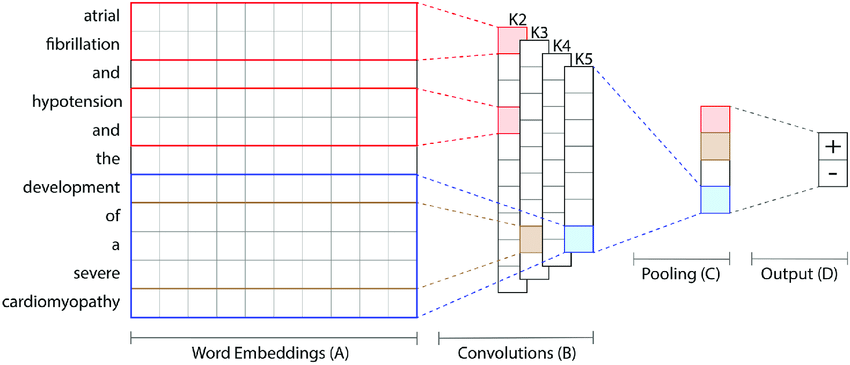
\includegraphics[width=350pt]{./Figures/cnn_overview.png}
        \caption{CNN 架構 \cite{gehrmann2018}}
        \label{fig:cnn_overview}
    \end{center}
\end{figure}

\section*{Result} 
\label{sec:Result}
\bookmark[level=chapter,page=\arabic{page}]{Result}

\subsection*{Simple Transformers}\bookmark[level=1,page=\arabic{page}]{Simple Transformers 結果}

Simple Transformers在public dataset的上傳紀錄以及每次參數設定示於 Table \ref{tab:simpletransformers_submission}。
針對每次上傳而得到的結果,採許相應的措施來提高F1-score 紀錄於 Table \ref{tab:reaction_sampletransformers}。
Simle Transformers同時會計算Training dataset與Testing dataset每個sample的長度,如 Figure \ref{fig:train_dataset_sentence_length}、Figure \ref{fig:test_dataset_sentence_length}。\\

\begin{longtable}{ccccc}
    \hline
    File          & Model   & Parameters                                                                                                                              & F1-score     & Note                                                                                                                                  \\ \hline \\
    \endfirsthead
    %
    \endhead
    %
    Submit1       & Roberta & \begin{tabular}[c]{@{}c@{}}Epoch=5\\   Learning\\   Rate:4e-5\\   BatchSize:8\\   max\_seq\_length:128\\   Threshold:0.5\end{tabular}   & 0.6346101231 & \begin{tabular}[c]{@{}c@{}}remove\\   stopwords\end{tabular}                                                                          \\ \\
    Submit2       & Roberta & \begin{tabular}[c]{@{}c@{}}Epoch=15\\   Learning\\   Rate:4e-5\\   BatchSize:16\\   max\_seq\_length:128\\   Threshold:0.5\end{tabular} & 0.6187086934 & \begin{tabular}[c]{@{}c@{}}remove\\   stopwords\end{tabular}                                                                          \\ \\
    Submit3       & Roberta & \begin{tabular}[c]{@{}c@{}}Epoch=20\\   Learning\\   Rate:4e-5\\   BatchSize:8\\   max\_seq\_length:128\\   Threshold:0.5\end{tabular}  & 0.6074731317 & \begin{tabular}[c]{@{}c@{}}remove\\   stopwords\end{tabular}                                                                          \\ \\
    Submit4       & Roberta & \begin{tabular}[c]{@{}c@{}}Epoch=10\\   Learning\\   Rate:4e-5\\   BatchSize:32\\   max\_seq\_length:256\\   Threshold:0.5\end{tabular} & 0.6197947699 & \begin{tabular}[c]{@{}c@{}}remove\\   stopwords\end{tabular}                                                                          \\ \\
    Submit5\_chen & Roberta & \begin{tabular}[c]{@{}c@{}}Epoch=7\\   Learning\\   Rate:4e-5\\   BatchSize:16\\   max\_seq\_length:70\\   Threshold:0.5\end{tabular}   & 0.6517648629 & \begin{tabular}[c]{@{}c@{}}without remove\\   stopwords\end{tabular}                                                                  \\ \\
    Submit5\_lin  & Roberta & \begin{tabular}[c]{@{}c@{}}Epoch=6\\   Learning\\   Rate:4e-5\\   BatchSize:16\\   max\_seq\_length:70\\   Threshold:0.4\end{tabular}   & 0.6614980112 & \begin{tabular}[c]{@{}c@{}}without remove\\   stopwords\end{tabular}                                                                  \\ \\
    Submit5\_lin2 & Roberta & \begin{tabular}[c]{@{}c@{}}Epoch=6\\   Learning\\   Rate:4e-5\\   BatchSize:16\\   max\_seq\_length:70\\   Threshold:0.3\end{tabular}   & 0.6317367309 & \begin{tabular}[c]{@{}c@{}}remove\\   stopwords\end{tabular}                                                                          \\ \\
    Submit6       & Roberta & \begin{tabular}[c]{@{}c@{}}Epoch=6\\   Learning\\   Rate:4e-5\\   BatchSize:16\\   max\_seq\_length:70\\   Threshold:0.3\end{tabular}   & 0.65423706   & \begin{tabular}[c]{@{}c@{}}without remove\\   stopwords\end{tabular}                                                                  \\ \\
    Submit7       & Roberta & \begin{tabular}[c]{@{}c@{}}Epoch=6\\   Learning\\   Rate:4e-5\\   BatchSize:16\\   max\_seq\_length:70\\   Threshold:0.4\end{tabular}   & 0.654321813  & \begin{tabular}[c]{@{}c@{}}without remove\\   stop words\\   if output皆小於threshold\\\{pred{[}max output value index{]}=1\}\end{tabular} \\ \\
    Submit9       & XLNet   & \begin{tabular}[c]{@{}c@{}}Epoch=7\\   Learning\\   Rate:4e-5\\   BatchSize:16\\   max\_seq\_length:70\\   Threshold:0.35\end{tabular}  & 0.6539460021 & \begin{tabular}[c]{@{}c@{}}without remove\\   stop words\\   if output皆小於threshold\\\{pred{[}max output value index{]}=1\}\end{tabular}\\ \\
    \caption{Simple Transformers 上傳紀錄}
    \label{tab:simpletransformers_submission}
\end{longtable}

\begin{figure}[H]
    \begin{minipage}[t]{0.5\textwidth}
    \begin{center}
        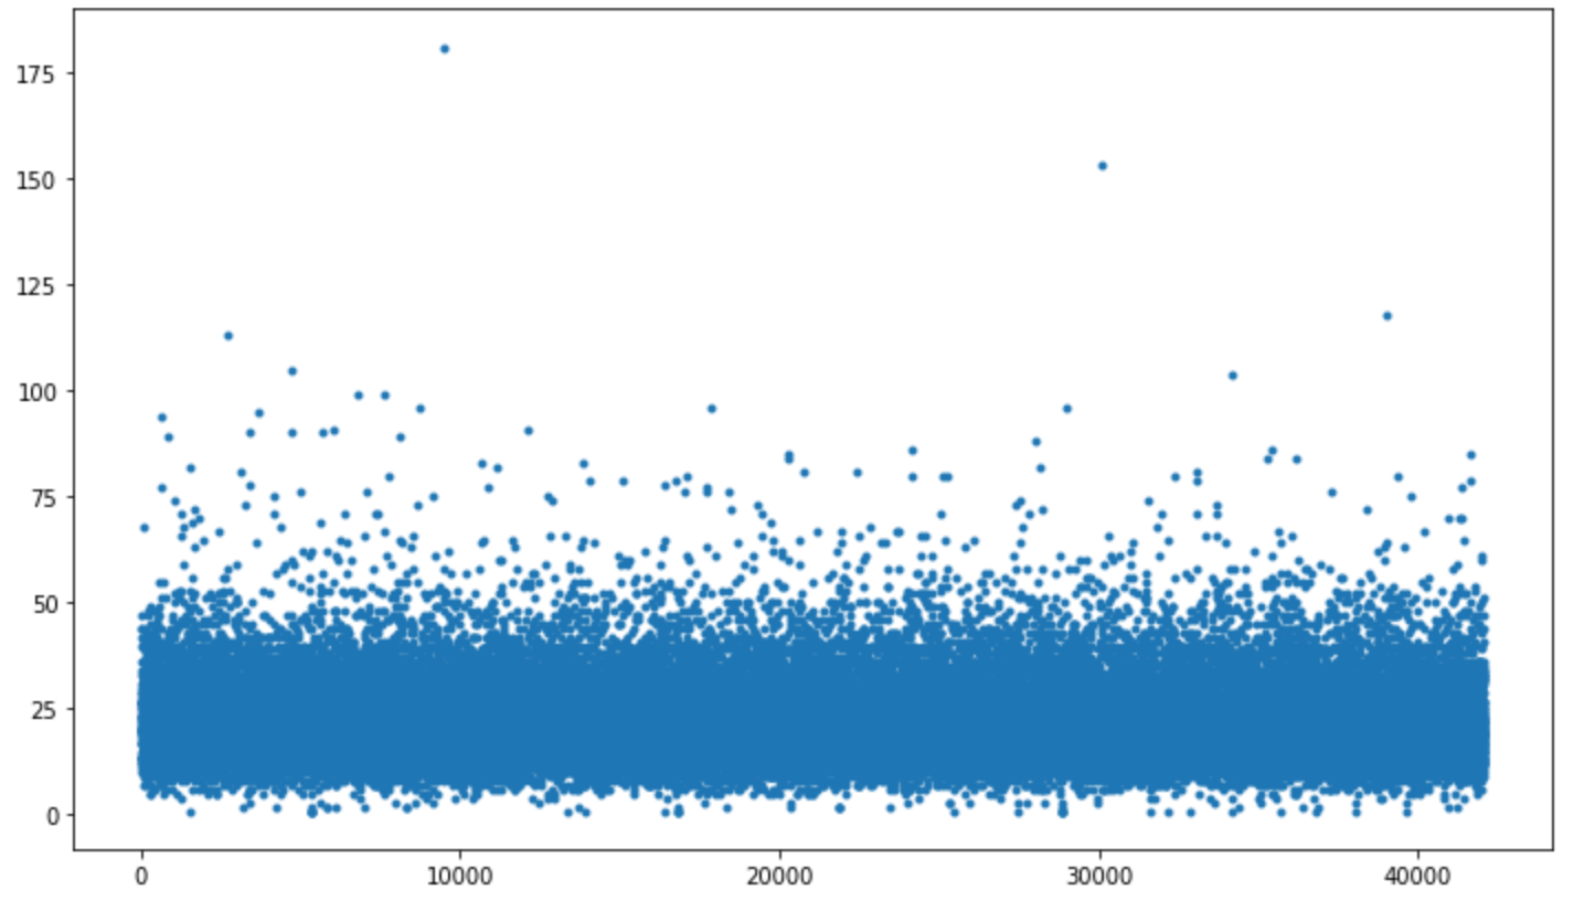
\includegraphics[width=190pt]{./Figures/train_dataset_sentence_length.png}
        \caption{Training dataset sentence length}
        \label{fig:train_dataset_sentence_length}
    \end{center}
    \end{minipage}
    \begin{minipage}[t]{0.5\textwidth}
        \begin{center}
            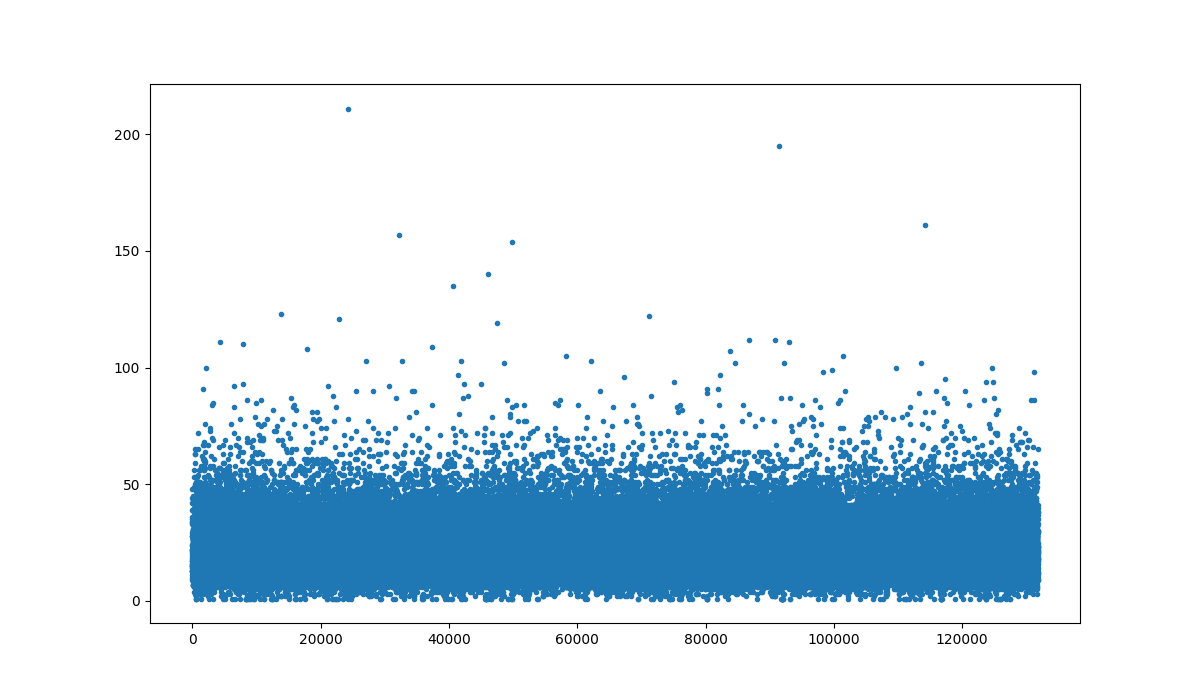
\includegraphics[width=215pt]{./Figures/test_dataset_sentence_length.png}
            \caption{Testing dataset sentence length}
            \label{fig:test_dataset_sentence_length}
        \end{center}
    \end{minipage}
\end{figure}   

\begin{table}[H]
    \centering
    \begin{tabular}{cc}
    \hline
    File & Result  \\ \hline \\
    Sumbit1-\textgreater{}Sumbit4    & train太多Epoch,acc下降         \\ \\
    Sumbit4-\textgreater{}Sumbit5    & Threshold和max\_seq\_length \\ \\
    Sumbit5\_2-\textgreater{}Sumbit6 & 比較有無 remove stopwords       \\ \\
    Submit7                          & 對fail的資料做後處理               \\ \\
    Submit9                          & 更換model                   
    \end{tabular}
    \caption{Simple Transformers 處理步驟}
    \label{tab:reaction_sampletransformers} 
\end{table}

\subsection*{Deep Learning Models} \bookmark[level=1,page=\arabic{page}]{Deep Learning Models 結果}

Deep Learning model中我們總共使用了CNN、RNN、RCNN、LSTM、GRU做測試。Table \ref{tab:deep_learning} 是我們找出每個model能夠達到的最高F1-score與當時設定的參數。
一開始發現即便增加CNN output channel 數量、word embedding dimension,CNN之F1-score仍然只於0.61左右,無法再向上提升,這時我們不得不考慮使用其他model。
但即使使用RNN、RCNN、LSTM,也從論文的建議使用directional RNN,F1-score都無法有顯著的提升。
還好回到GRU後嘗試增加number of layers,F1-score才發生了明顯的進步。我們這組在LeaderBoard上的排名從100多名直接跳躍至第37名。\\

正式比賽當天採用GRU的F1-score與Loss隨著Epoch增加而變化的曲線圖如 Figure \ref{fig:F1_GRU} 與 Figure \ref{fig:Loss_GRU} 所示。
為了避免overfitting的情況發生,用於預測testing dataset的model選validation dataset中F1-score最高的epoch所訓練的model。
也因為有validation dataset的存在,上傳public dataset時即使看不見F1-score,也能以我們所訓練出最好的model作最後一次上傳依據。\\

\begin{longtable}{cccc}
    \hline
    Model & Best F1-score & Best Epoch & Note
    \endfirsthead
    %
    \endhead
    %
    \hline \\
    CNN & 0.61003 & 36 & \begin{tabular}[c]{@{}c@{}}embedding\_dim = 300\\ hidden\_dim = 512\\ learning\_rate = 1e-5\\ max\_epoch = 50\\ batch\_size = 16\end{tabular} \\ \\
    RNN & 0.60374 & 8 & \begin{tabular}[c]{@{}c@{}}embedding\_dim = 300\\ hidden\_dim = 1000\\ learning\_rate = 1e-5\\ max\_epoch = 50\\ batch\_size = 15\\ num\_layers=2\end{tabular} \\ \\
    RCNN & 0.62694 & 25 & \begin{tabular}[c]{@{}c@{}}embedding\_dim = 300\\ hidden\_dim = 1000\\ learning\_rate = 1e-5\\ max\_epoch = 50\\ batch\_size = 32\\ num\_layers=2\end{tabular} \\ \\
    LSTM & 0.62294 & 47 & \begin{tabular}[c]{@{}c@{}}embedding\_dim = 300\\ hidden\_dim = 1000\\ learning\_rate = 1e-5\\ max\_epoch = 50\\ batch\_size = 15\\ num\_layers = 2\end{tabular} \\ \\
    GRU & 0.69592 & 44 & \begin{tabular}[c]{@{}c@{}}embedding\_dim = 100\\ hidden\_dim = 512\\ learning\_rate = 1e-4\\ max\_epoch = 50\\ batch\_size = 16\\ num\_layers = 2\end{tabular} \\
    \caption{Deep Learning Model 測試結果}\\
    \label{tab:deep_learning}
\end{longtable}


\begin{comment} %This is good
\begin{figure}[H]
    \centering
    \subfigure[name1]{
    \label{Fig.sub.1}
    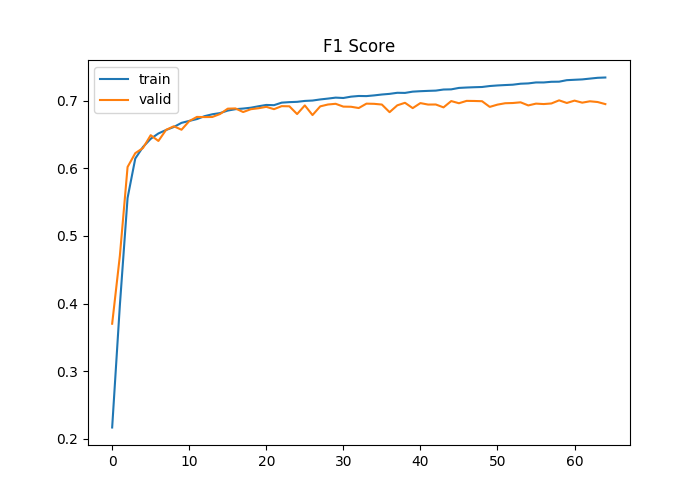
\includegraphics[width=0.45\textwidth]{./Figures/F1_score_GRU.png}}
    \subfigure[name2]{
    \label{Fig.sub.2}
    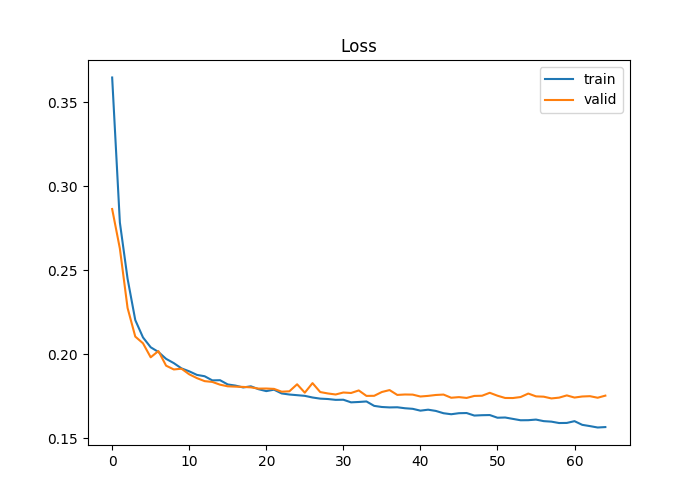
\includegraphics[width=0.45\textwidth]{./Figures/Loss_sample_GRU.png}}
    \caption{Main name}
    \label{Fig.main}
\end{figure}
\end{comment}

\begin{figure}[H]
    \begin{minipage}[t]{0.5\textwidth}
    \begin{center}
        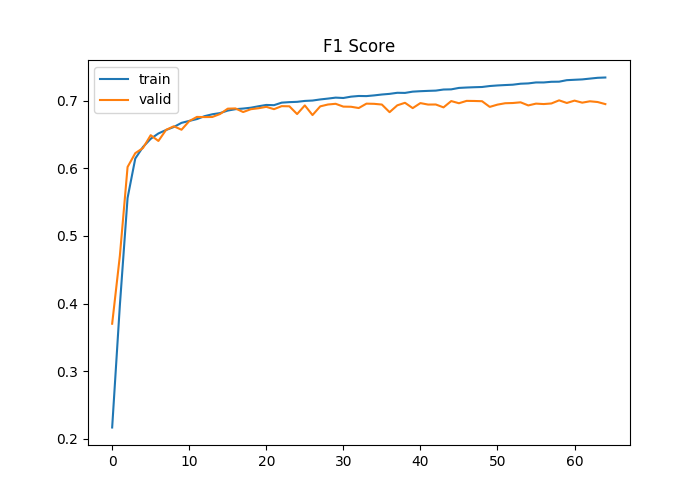
\includegraphics[width=250pt]{./Figures/F1_score_GRU.png}
        \caption{F1 score from GRU}
        \label{fig:F1_GRU}
    \end{center}    
    \end{minipage}    
    \begin{minipage}[t]{0.5\textwidth}
    \begin{center}
        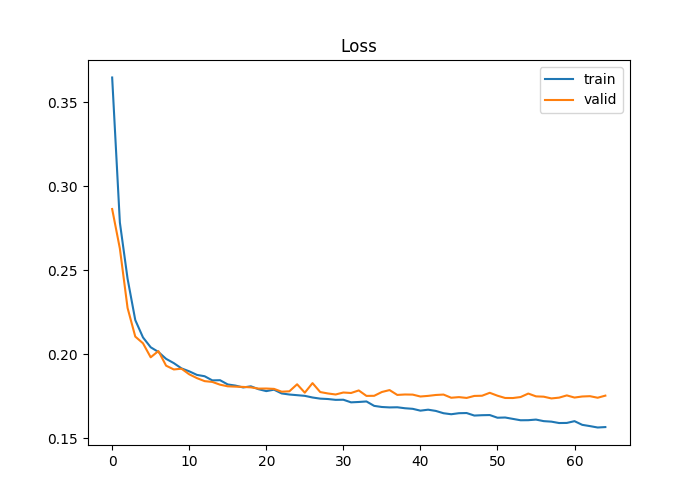
\includegraphics[width=250pt]{./Figures/Loss_sample_GRU.png}
        \caption{Loss from GRU}
        \label{fig:Loss_GRU}
    \end{center}    
    \end{minipage}
\end{figure}

%\colorbox{green}{CNN、LSTM、RNN、GRU 比較表格}

\section*{Discussion} 
\label{sec:Discussion}
\bookmark[level=chapter,page=\arabic{page}]{Discussion}

\subsection*{林睿哲個人心得}
\bookmark[level=1,page=\arabic{page}]{林睿哲個人心得}

這次人工智慧論文標註競賽,是我第一次參加與人工智慧相關的比賽,雖然之前已經接觸過一些有關人工智慧的相關技術,但多半都是與電腦視覺相關,這次的比賽是我第一次接觸自然語言處理,一開始相當無助,完全不知道該如何下手,經過不斷上網看資料及教學影片,才漸漸理解一些有關NLP的相關知識,從RNN的LSTM和GRU到word embeddings,再到最新的Self Attention和Transformer,花了好幾個星期才稍微了解NLP的處理流程及細節。一開始我們先選擇了Roberta,它算是相當新的技術,在2019年中才被Facebook提出,過程中,我們不斷嘗試不一樣的parameters,像是發現train太多epoch會導致model過度學習,又或者是threshold對multilabel分類問題,是相當重要的一個環節,同時我們也對原始資料進行分析,發現每個句子的長度多半在70上下,因此後面我們也將最大句子長度改為70,也對準確度有所提升。除了分析原始資料我們也對預測失敗的資料進行分析,雖然有慢慢提升accuracy,但始終沒辦法跨越0.66,也證明了最新的技術,不代表一定適合我們的資料。於是我們回頭研究傳統的CNN及RNN,從CNN的character embedding到RNN的LSTM及GRU,最後發現在GRU方面效果意外的好,比賽當天也使用GRU在Private Dataset中突破0.69,獲得0.7033732的成績,排名17/78。\\

透過參加這次比賽,除了對自然語言處理有初步認識外,也體會到參數調整所帶來的挫折,常常train了好幾小時,準確度卻只上升千分之一,甚至有時候不升反降,但在這過程中,我更了解這些參數所扮演的不同角色,此外也讓我學習到如何對一筆資料進行分析,去獲得一些有助於提升預測準確度的資訊。這次比賽距離得名只差了7名,準確度也只差了0.012968,但我深刻體會到為了提升這0.01其實要付出很大的努力,雖然這次比賽沒有得名,但我相信透過實作的方式,比起期末考試,更讓我獲益良多。 \\

\subsection*{陳誼家個人心得}
\bookmark[level=1,page=\arabic{page}]{陳誼家個人心得}

這次的比賽對我來說難度有點高。原因是本來就對 deep learning 的建模方式不甚熟悉,再加上此次比賽又是之前沒有接觸過的 NLP 問題,許多技術與名詞都是第一次聽到,或是曾有聽過可是從沒去真正了解那是什麼,像是 RNN、glove, 甚至 LSTM 和 BERT。所幸主辦單位與助教有提供 sample code。不過搞懂 sample code 也是花了我不少時間。沒接觸過 NLP 問題,也導致我在面對資料預處理的時候很沒有頭緒。也幸虧可以透過各組的報告時間,聽取其他組別在資料預處理上的一些眉眉角角,甚至是不適合的做法。例如,如果要使用 BERT,因為它會根據一個字在一個句子中的位置來判斷字的意思,所以每個字都有存在的必要,不能任意地拿掉 stop words。這個是我之前沒有想過的問題,儘管已經查詢過 BERT 的相關資訊。其他的像是透過將句子翻譯成中文再翻譯回來英文,以得到更多的 training data,或是拿另一個 task 的資料,還有針對每個 label 獨立訓練「是與否」的model,最後再將所有的 label 訓練結果整合起來。這些都是在聽到各組分享前沒有想到過的。不過,我們最後採用的model還是 GRU。這邊真的要感謝隊友,沒有他沒日沒夜地嘗試各種model與資料預處理的方式,並且調整各種參數,我們才有辦法在最終結果突破 70 分大關。\\

總而言之,此次的比賽讓我接觸到了一塊以前沒涉略的 NLP,同時也是第一次參加這麼大型的競賽。第一次上傳我們的 public test set 時,在 leader board 上看到這麼多組別排在我們前面,但是彼此分數卻又非常相近,不僅讓我了解比賽當中,每個小細節其實都非常重要,也深深了解到自己這方面能力的不足。\\


\subsection*{伍錫志個人心得}
\bookmark[level=1,page=\arabic{page}]{伍錫志個人心得}

首先要感謝機械系\href{https://nckunclab.wixsite.com/neuralcomputationlab}{神經計算實驗室}提供
伺服器 (Figure \ref{fig:our_GPU}) 與個人電腦 (Figure \ref{fig:my_GPU}),是運算的主力工具。
比賽前兩周更是每天必須同時間使用三台電腦測試跑測試,才能從堆積如山的model中找出最佳參數。
從實作方面來說,這是我第一次成功使用Neural Network model。從GPU運算環境架設、學習Docker與Pytorch,這個競賽所需要的技術非常龐大且複雜。
從網路上找到的\href{https://www.tensorflow.org/install/docker}{Docker教學}與\href{https://github.com/zergtant/pytorch-handbook}{Pytorch教學}一
步步累積技術,
在分秒必爭的競賽時程內,如何快速部屬程式碼到不同的電腦上、使用GPU作加速運算、詳細的git版本管理都是會左右賽局的關鍵,也是我認為最後打敗其他團隊的致勝原因。\\

其實一開始有相當多的時間是在整理input data。雖然Sample Code已經提供讀入csv檔、nltk資料前處理、train-test split等功能,
但是我缺乏的關鍵步驟:拆解sample使的每個sample只會對應到一個label。這個簡單的功能耗費了將近1周才完成,
不過是在成功的得到這個input data格式後,才能讓我順利運行眾多經典Neural Network model。
從理論方面來說,是在發現原本預期使用CNN model無法達到baseline標準,才回頭找相關論文研究。
除了參考論文中Neural Network架構是如何設計的,更需要了解每個model的特性與差異,用最有效率的方式調整參數。
例如CNN的訓練時間比LSTM快速、LSTM 對batch size很敏感,若sample數量無法整除則無法訓練...等。透過這次實際操作讓我對這些Neural Network model有深入的了解。
更重要的是,體會到作研究不能閉門造車,一定要先作廣泛的文獻探討。如果發現原本的方法行不通或是無法達到預期水準,
有可能是操作有誤,抑或是由於資料型態的不同導致。這時除了檢查自己的程式碼與論文提出的架構做比較之外,
找到下一個合適的方式也是需要納入考慮。現在回頭看,或許是因為做句子標註受限於每個sample篇幅很短,
導致CNN這個方式無法有效的完成準確的標註任務。\\

經過這次實戰,讓我對於技術、理論都有了更進一步的體驗。唯有透過技術與理論的相輔相成,
追求突破才不會令人感到遙不可及。

    % \begin{figure}[H]
    %     \begin{center}
    %         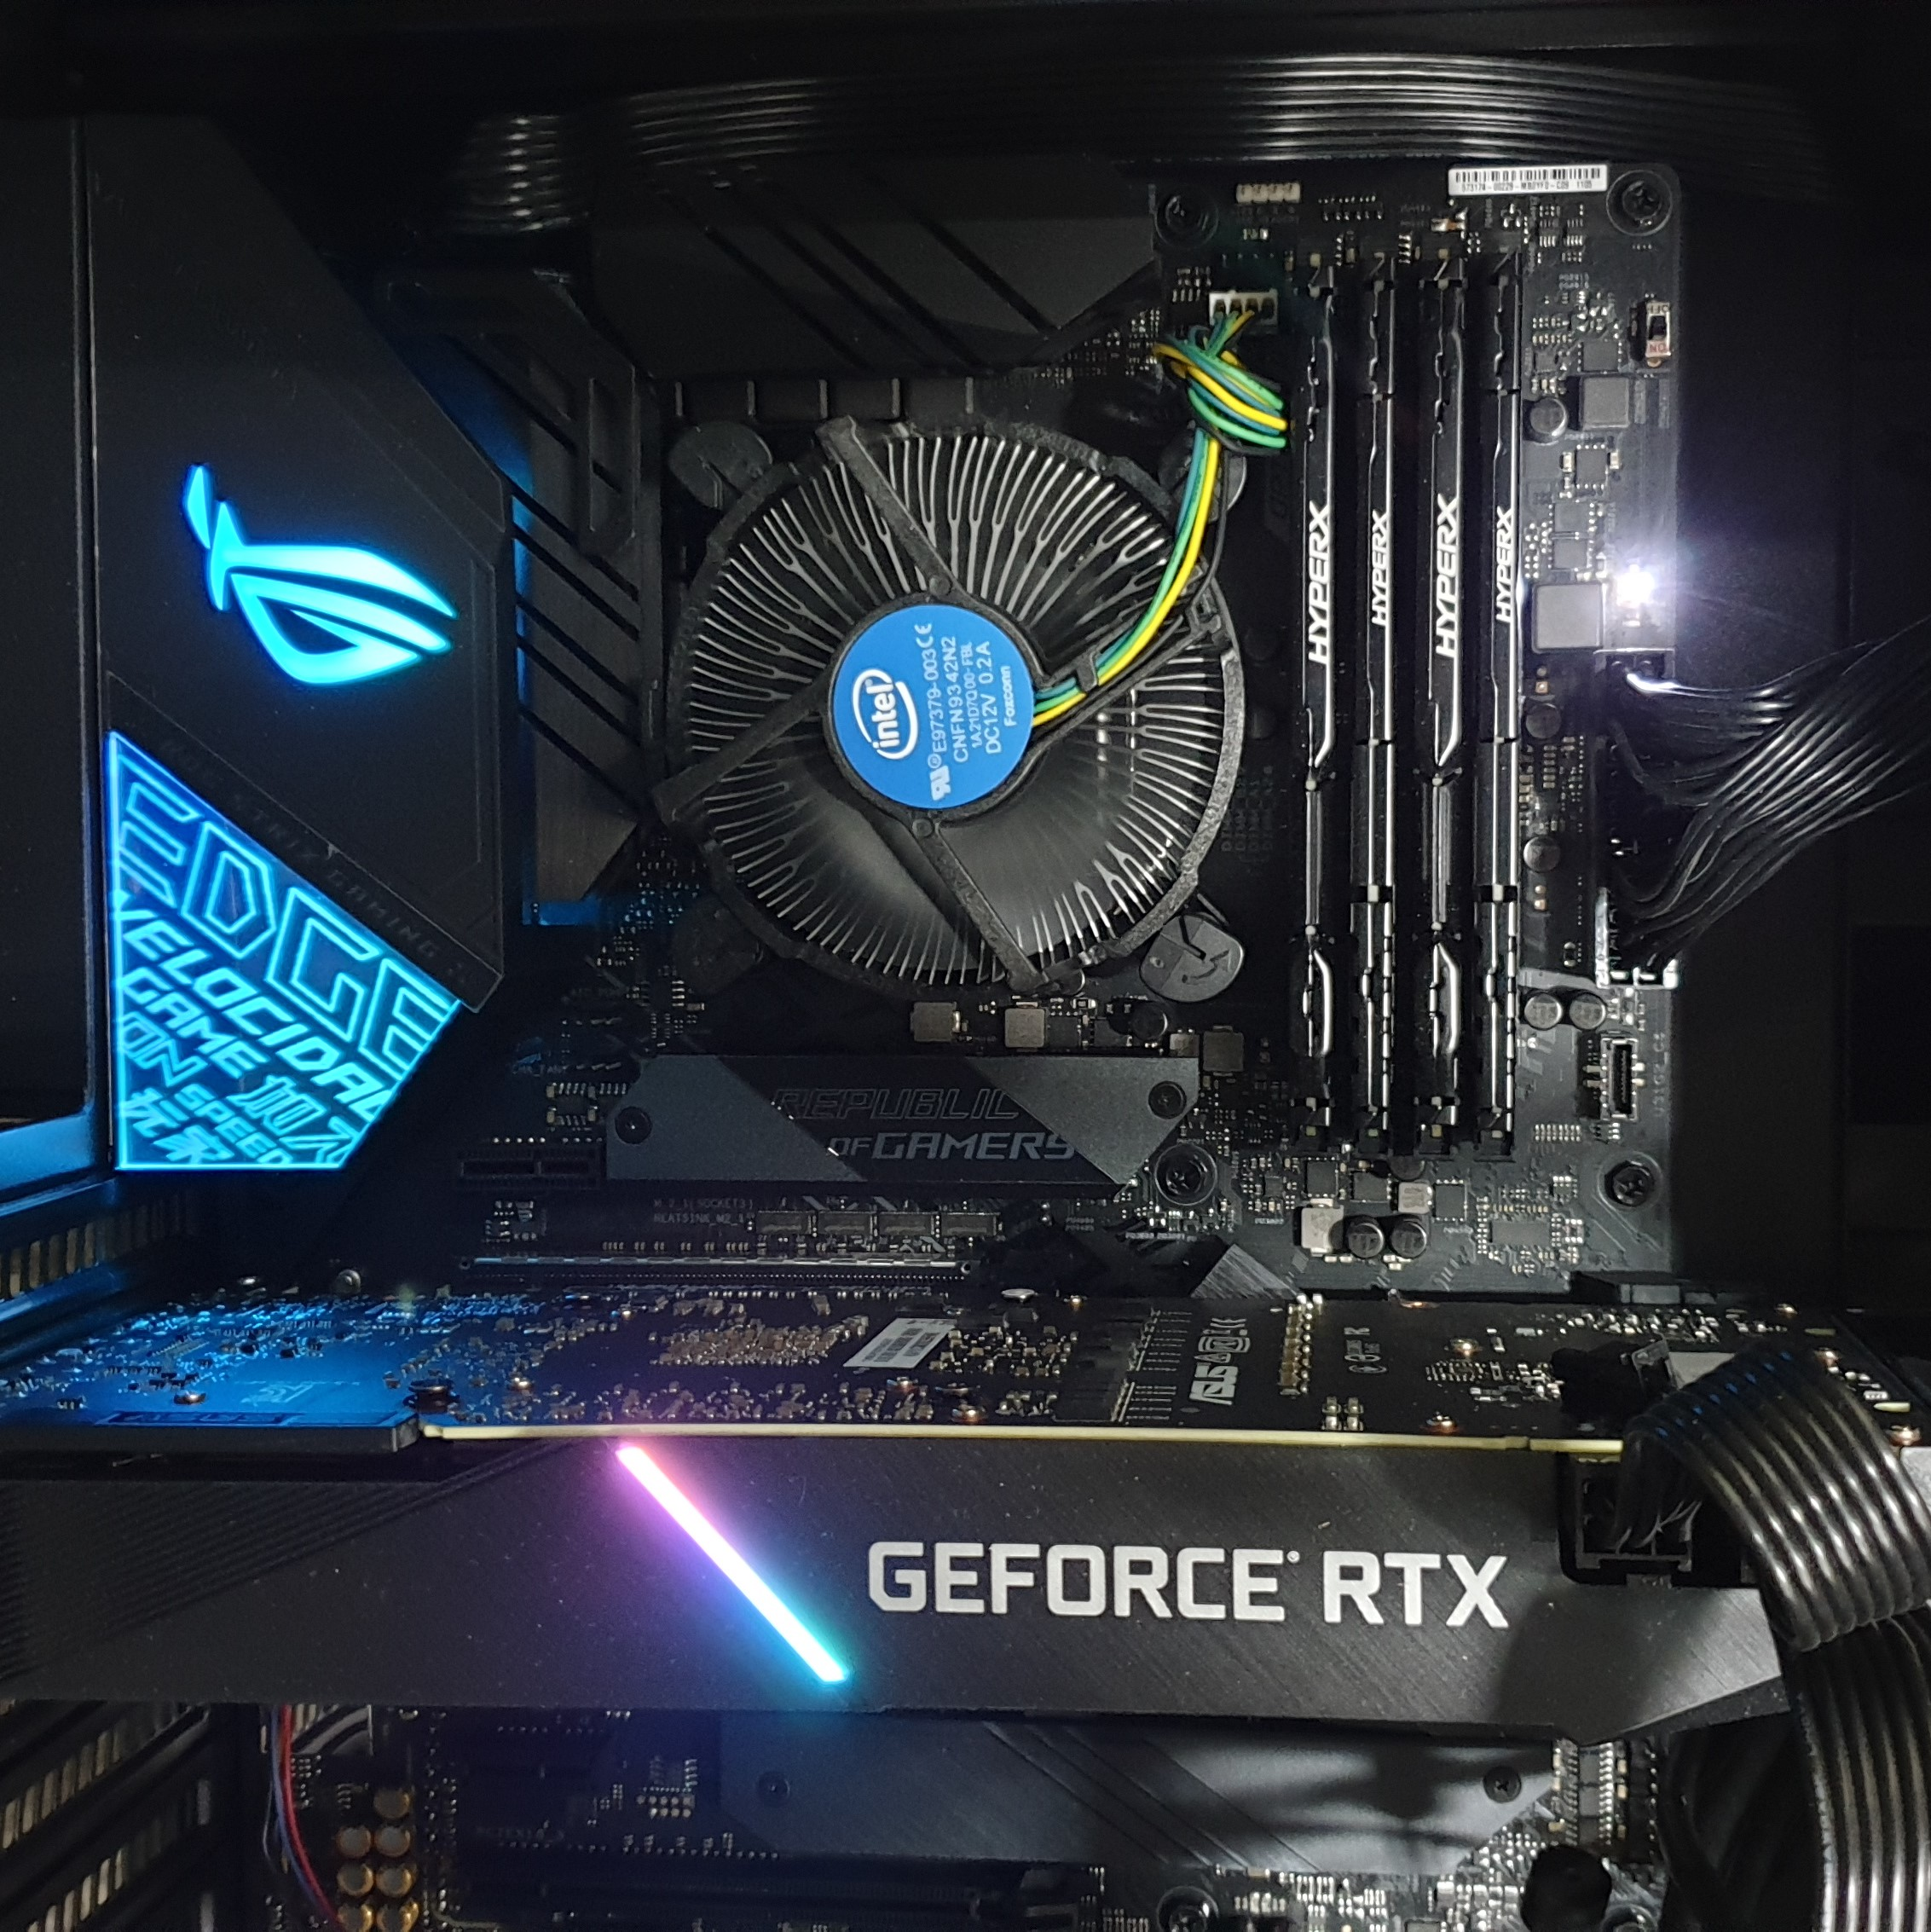
\includegraphics[width=250pt]{./Figures/RTX2070s.jpg}
    %         \caption{硬體設備\\Intel(R) Core(TM) i7-9700 CPU\\RTX2070s GPU}
    %         \label{fig:our_GPU}
    %     \end{center}
    % \end{figure}

\begin{figure}[H]
    \begin{minipage}[t]{0.5\textwidth}
    \begin{center}
        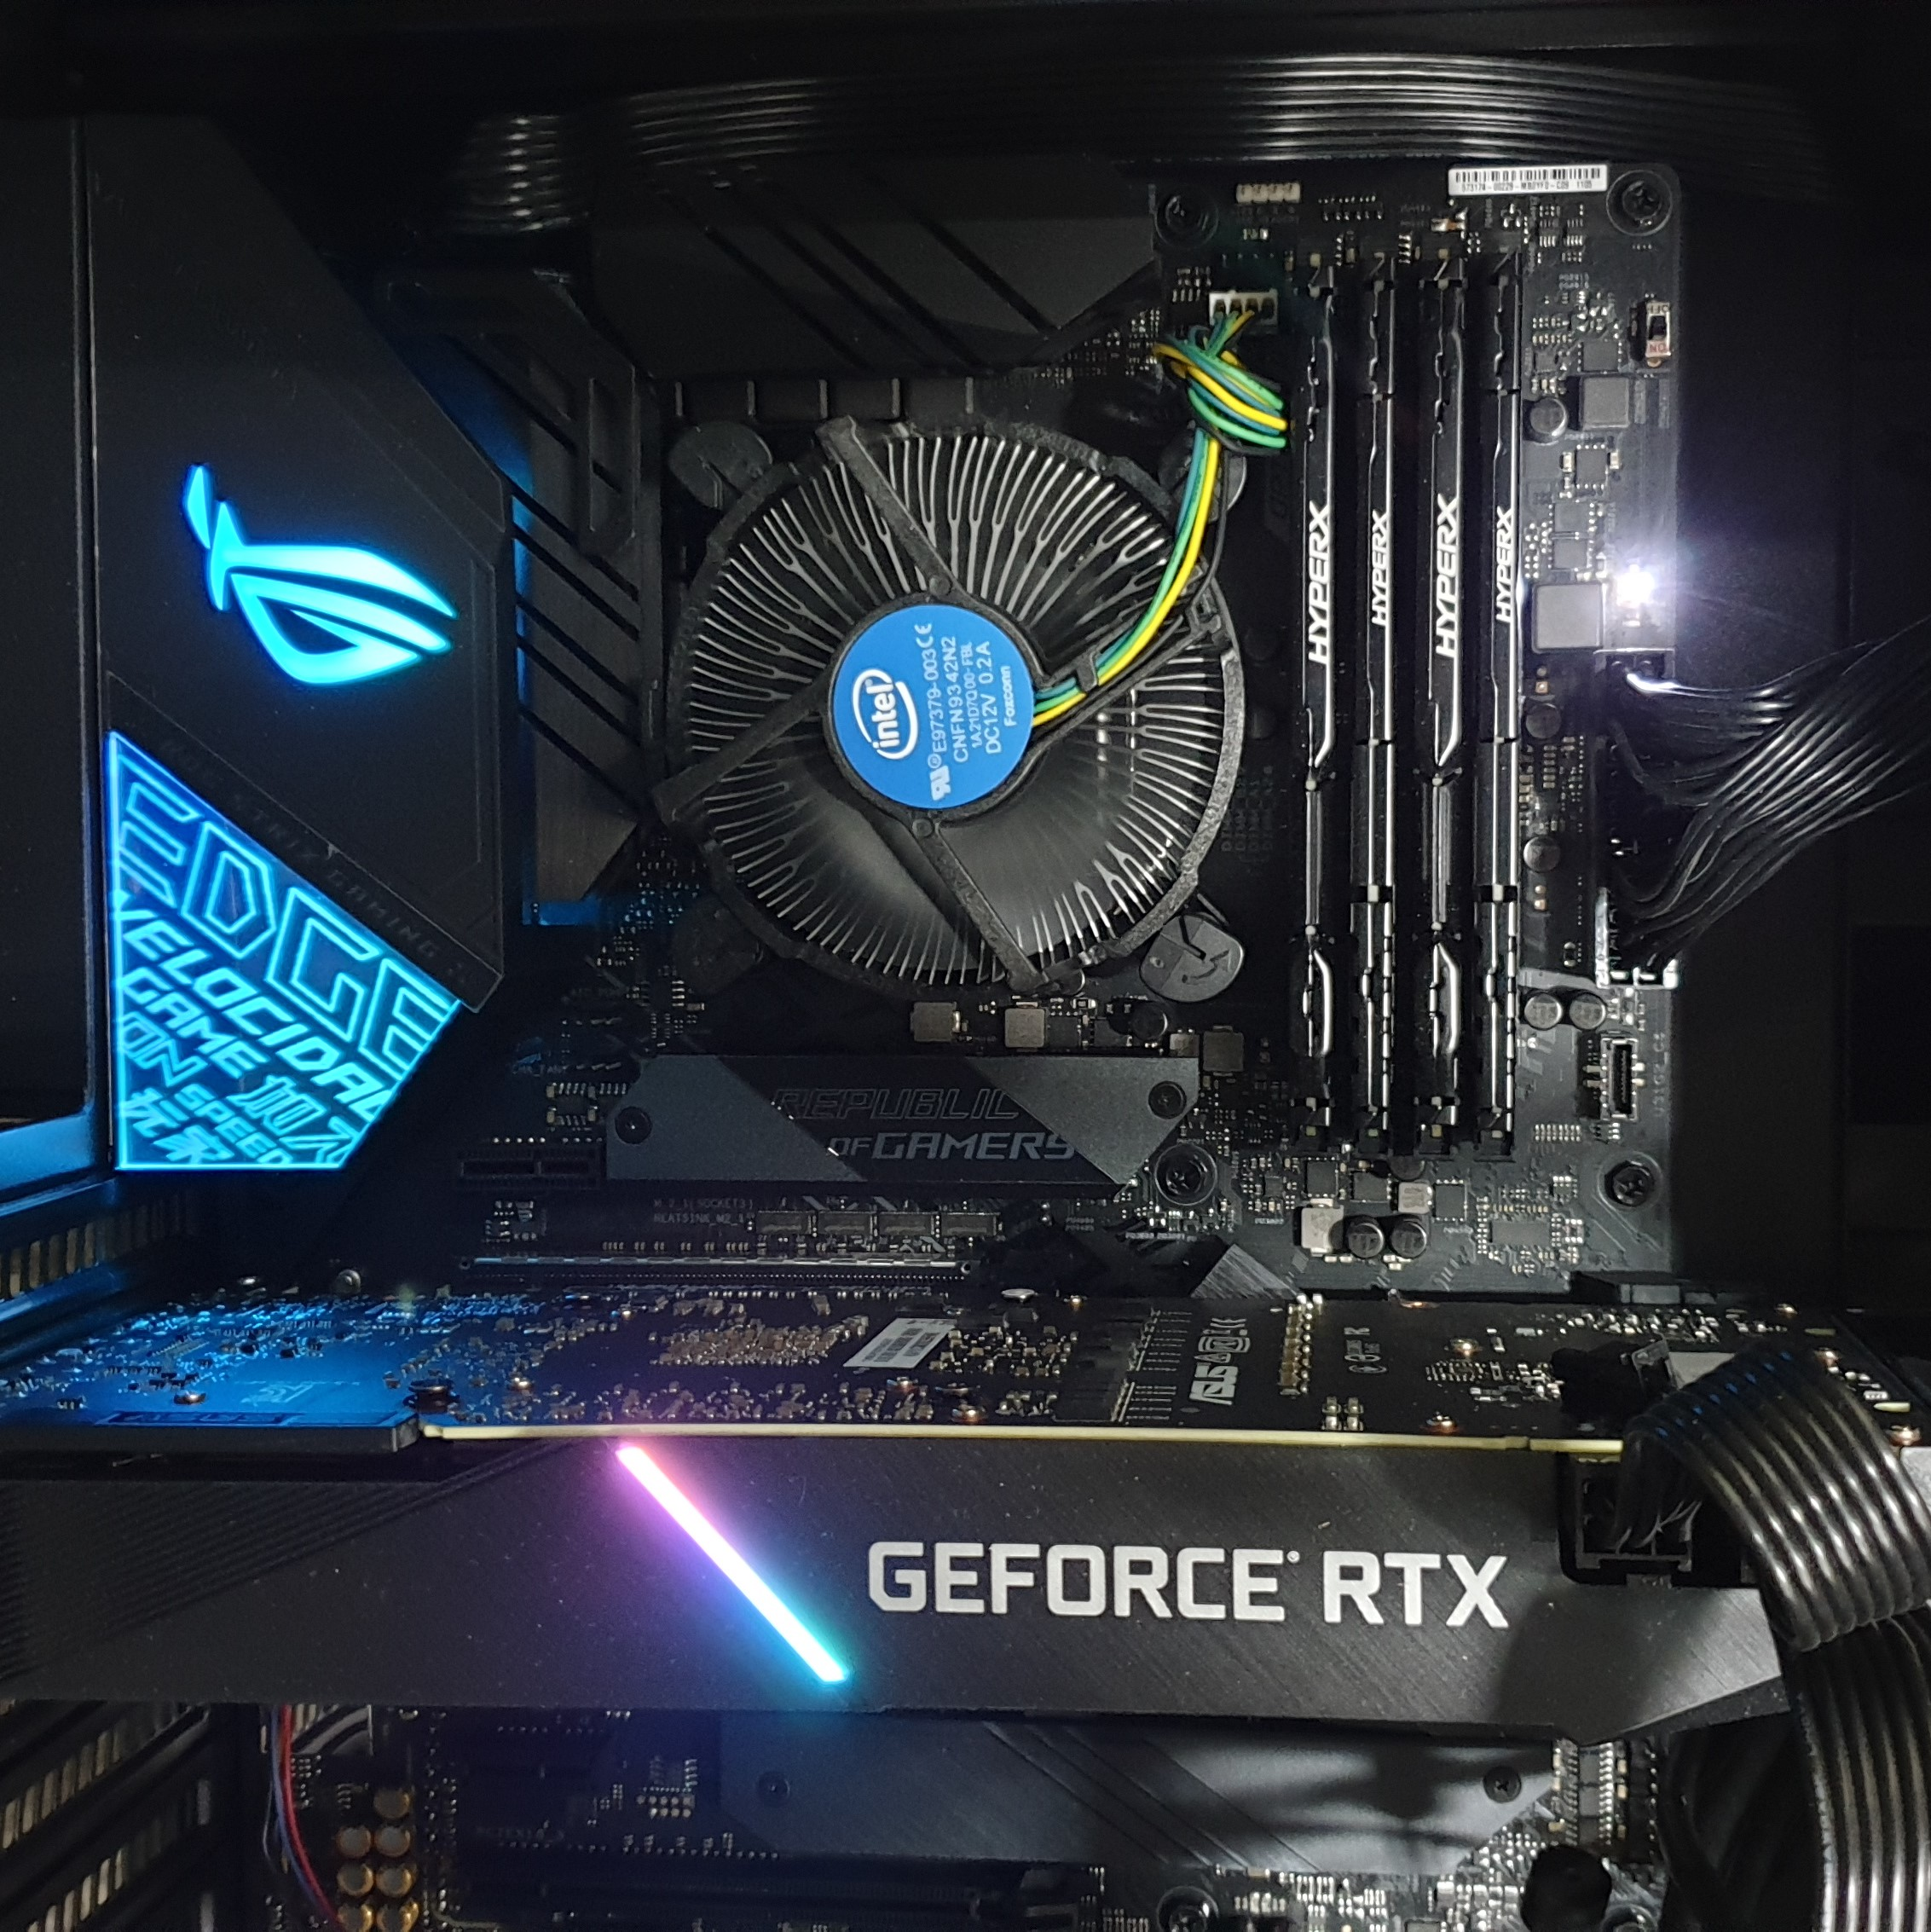
\includegraphics[width=220pt]{./Figures/RTX2070s}
        \caption{Intel i7-9700 CPU, RTX2070s GPU}
        \label{fig:our_GPU}
    \end{center}    
    \end{minipage}    
    \begin{minipage}[t]{0.5\textwidth}
    \begin{center}
        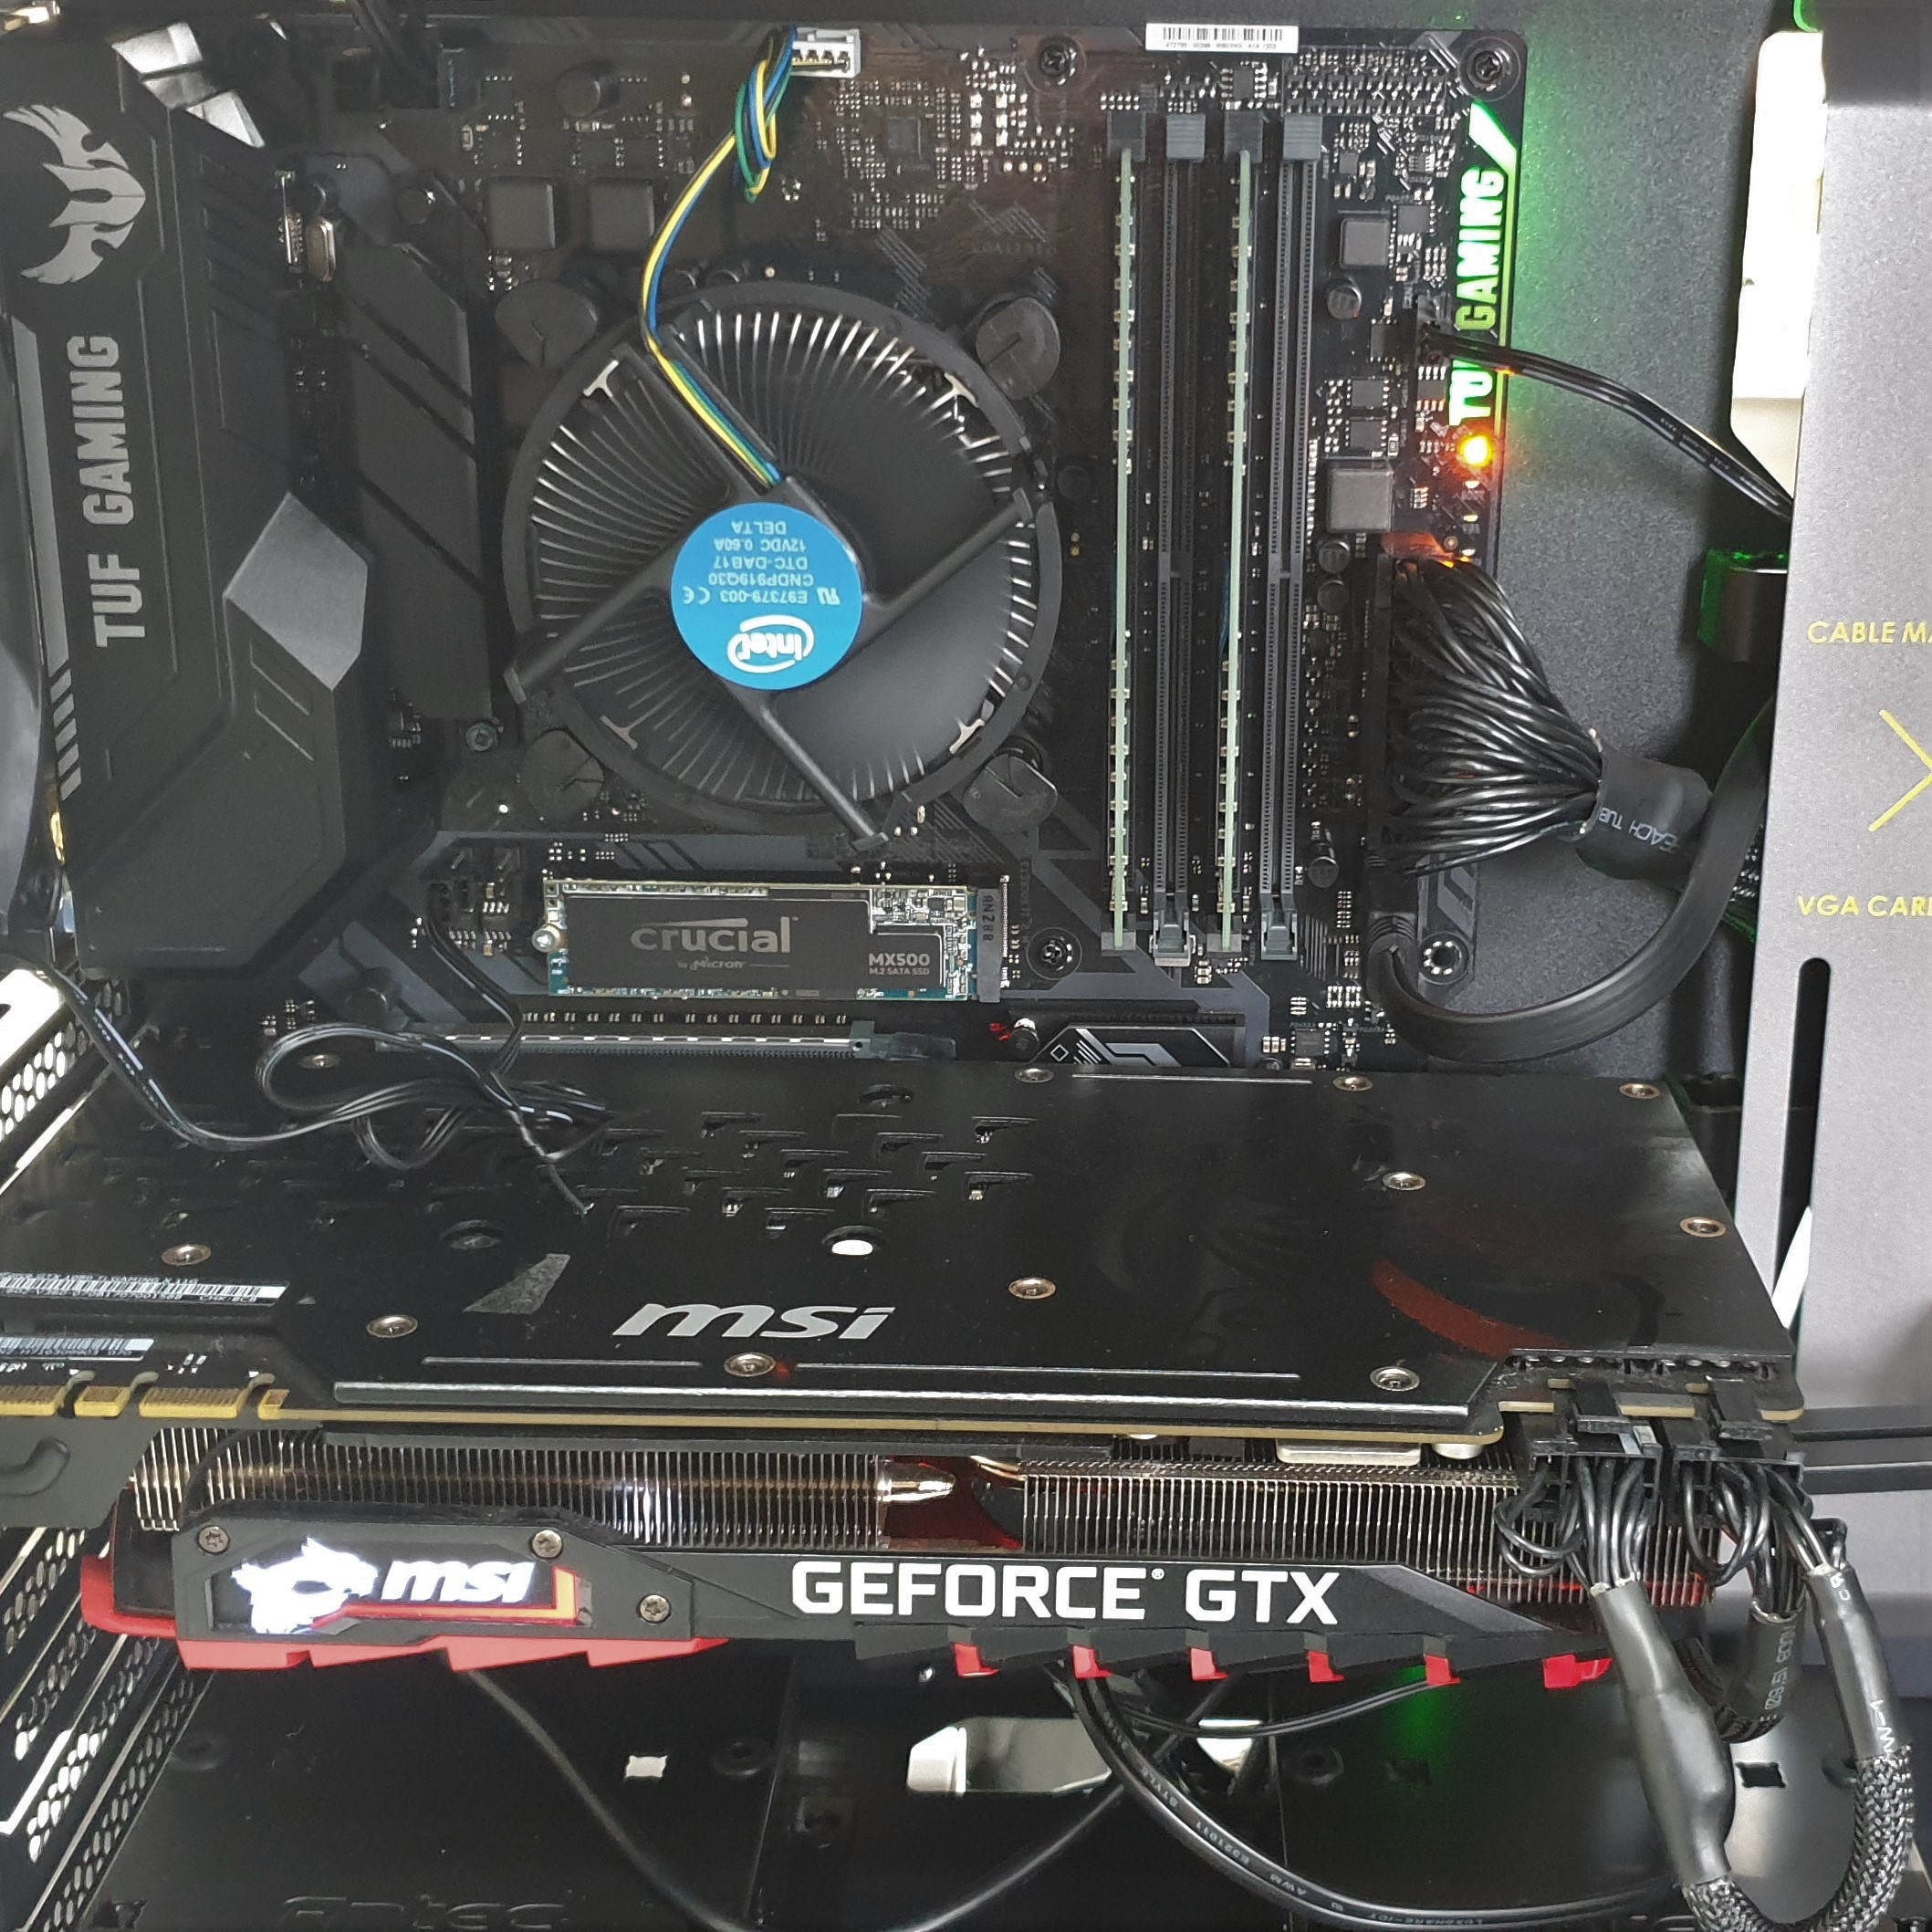
\includegraphics[width=220pt]{./Figures/GTX1080Ti.jpg}
        \caption{Intel i5-9400 CPU, GTX1080Ti GPU}
        \label{fig:my_GPU}
    \end{center}    
    \end{minipage}
\end{figure}


\section*{Conclusion} 
\label{sec:Conclusion}
\bookmark[level=chapter,page=\arabic{page}]{Conclusion}

最終使用GRU為比賽model,得到相當不錯的成績,也超越baseline(0.69)。上傳 private dataset 的期間竟然無法得知我們上傳預測結果的F1 score,
這讓許多參賽者相當苦惱。還好有將 training data 挑出 validation set,讓我們能夠挑選出最適當的 epoch 與 model,不至於盲目上傳預測結果。
相較於傳統NLP技術,stopwords有助於Neural Network訓練,不同model在不去除stopwords的情況下約可上升約5\%左右的F1-score;Lemmatization則是可有可無。\\

經過這次實作的經驗,讓我們知道當遇見瓶頸時,參考研究論文是一件非常重要而有效率的方式。不但可以學習他人研究精華,也節省不少盲目測試的時間。
同時也察覺到現有Neural Network相關套件、model所不足之處,值得繼續研究改進。

\bookmark[level=chapter,page=\arabic{page}]{References}
\bibliography{./reference} \label{sec:references}
\newpage

\end{document}